% Options for packages loaded elsewhere
\PassOptionsToPackage{unicode}{hyperref}
\PassOptionsToPackage{hyphens}{url}
%
\documentclass[
  ignorenonframetext,
  aspectratio=169,
]{beamer}
\usepackage{pgfpages}
\setbeamertemplate{caption}[numbered]
\setbeamertemplate{caption label separator}{: }
\setbeamercolor{caption name}{fg=normal text.fg}
\beamertemplatenavigationsymbolshorizontal
% Prevent slide breaks in the middle of a paragraph
\widowpenalties 1 10000
\raggedbottom
\setbeamertemplate{part page}{
  \centering
  \begin{beamercolorbox}[sep=16pt,center]{part title}
    \usebeamerfont{part title}\insertpart\par
  \end{beamercolorbox}
}
\setbeamertemplate{section page}{
  \centering
  \begin{beamercolorbox}[sep=12pt,center]{part title}
    \usebeamerfont{section title}\insertsection\par
  \end{beamercolorbox}
}
\setbeamertemplate{subsection page}{
  \centering
  \begin{beamercolorbox}[sep=8pt,center]{part title}
    \usebeamerfont{subsection title}\insertsubsection\par
  \end{beamercolorbox}
}
\AtBeginPart{
  \frame{\partpage}
}
\AtBeginSection{
  \ifbibliography
  \else
    \frame{\sectionpage}
  \fi
}
\AtBeginSubsection{
  \frame{\subsectionpage}
}

\usepackage{amsmath,amssymb}
\usepackage{iftex}
\ifPDFTeX
  \usepackage[T1]{fontenc}
  \usepackage[utf8]{inputenc}
  \usepackage{textcomp} % provide euro and other symbols
\else % if luatex or xetex
  \usepackage{unicode-math}
  \defaultfontfeatures{Scale=MatchLowercase}
  \defaultfontfeatures[\rmfamily]{Ligatures=TeX,Scale=1}
\fi
\usepackage{lmodern}
\ifPDFTeX\else  
    % xetex/luatex font selection
\fi
% Use upquote if available, for straight quotes in verbatim environments
\IfFileExists{upquote.sty}{\usepackage{upquote}}{}
\IfFileExists{microtype.sty}{% use microtype if available
  \usepackage[]{microtype}
  \UseMicrotypeSet[protrusion]{basicmath} % disable protrusion for tt fonts
}{}
\usepackage{xcolor}
\newif\ifbibliography
\setlength{\emergencystretch}{3em} % prevent overfull lines
\setcounter{secnumdepth}{-\maxdimen} % remove section numbering

\usepackage{color}
\usepackage{fancyvrb}
\newcommand{\VerbBar}{|}
\newcommand{\VERB}{\Verb[commandchars=\\\{\}]}
\DefineVerbatimEnvironment{Highlighting}{Verbatim}{commandchars=\\\{\}}
% Add ',fontsize=\small' for more characters per line
\usepackage{framed}
\definecolor{shadecolor}{RGB}{241,243,245}
\newenvironment{Shaded}{\begin{snugshade}}{\end{snugshade}}
\newcommand{\AlertTok}[1]{\textcolor[rgb]{0.68,0.00,0.00}{#1}}
\newcommand{\AnnotationTok}[1]{\textcolor[rgb]{0.37,0.37,0.37}{#1}}
\newcommand{\AttributeTok}[1]{\textcolor[rgb]{0.40,0.45,0.13}{#1}}
\newcommand{\BaseNTok}[1]{\textcolor[rgb]{0.68,0.00,0.00}{#1}}
\newcommand{\BuiltInTok}[1]{\textcolor[rgb]{0.00,0.23,0.31}{#1}}
\newcommand{\CharTok}[1]{\textcolor[rgb]{0.13,0.47,0.30}{#1}}
\newcommand{\CommentTok}[1]{\textcolor[rgb]{0.37,0.37,0.37}{#1}}
\newcommand{\CommentVarTok}[1]{\textcolor[rgb]{0.37,0.37,0.37}{\textit{#1}}}
\newcommand{\ConstantTok}[1]{\textcolor[rgb]{0.56,0.35,0.01}{#1}}
\newcommand{\ControlFlowTok}[1]{\textcolor[rgb]{0.00,0.23,0.31}{\textbf{#1}}}
\newcommand{\DataTypeTok}[1]{\textcolor[rgb]{0.68,0.00,0.00}{#1}}
\newcommand{\DecValTok}[1]{\textcolor[rgb]{0.68,0.00,0.00}{#1}}
\newcommand{\DocumentationTok}[1]{\textcolor[rgb]{0.37,0.37,0.37}{\textit{#1}}}
\newcommand{\ErrorTok}[1]{\textcolor[rgb]{0.68,0.00,0.00}{#1}}
\newcommand{\ExtensionTok}[1]{\textcolor[rgb]{0.00,0.23,0.31}{#1}}
\newcommand{\FloatTok}[1]{\textcolor[rgb]{0.68,0.00,0.00}{#1}}
\newcommand{\FunctionTok}[1]{\textcolor[rgb]{0.28,0.35,0.67}{#1}}
\newcommand{\ImportTok}[1]{\textcolor[rgb]{0.00,0.46,0.62}{#1}}
\newcommand{\InformationTok}[1]{\textcolor[rgb]{0.37,0.37,0.37}{#1}}
\newcommand{\KeywordTok}[1]{\textcolor[rgb]{0.00,0.23,0.31}{\textbf{#1}}}
\newcommand{\NormalTok}[1]{\textcolor[rgb]{0.00,0.23,0.31}{#1}}
\newcommand{\OperatorTok}[1]{\textcolor[rgb]{0.37,0.37,0.37}{#1}}
\newcommand{\OtherTok}[1]{\textcolor[rgb]{0.00,0.23,0.31}{#1}}
\newcommand{\PreprocessorTok}[1]{\textcolor[rgb]{0.68,0.00,0.00}{#1}}
\newcommand{\RegionMarkerTok}[1]{\textcolor[rgb]{0.00,0.23,0.31}{#1}}
\newcommand{\SpecialCharTok}[1]{\textcolor[rgb]{0.37,0.37,0.37}{#1}}
\newcommand{\SpecialStringTok}[1]{\textcolor[rgb]{0.13,0.47,0.30}{#1}}
\newcommand{\StringTok}[1]{\textcolor[rgb]{0.13,0.47,0.30}{#1}}
\newcommand{\VariableTok}[1]{\textcolor[rgb]{0.07,0.07,0.07}{#1}}
\newcommand{\VerbatimStringTok}[1]{\textcolor[rgb]{0.13,0.47,0.30}{#1}}
\newcommand{\WarningTok}[1]{\textcolor[rgb]{0.37,0.37,0.37}{\textit{#1}}}

\providecommand{\tightlist}{%
  \setlength{\itemsep}{0pt}\setlength{\parskip}{0pt}}\usepackage{longtable,booktabs,array}
\usepackage{calc} % for calculating minipage widths
\usepackage{caption}
% Make caption package work with longtable
\makeatletter
\def\fnum@table{\tablename~\thetable}
\makeatother
\usepackage{graphicx}
\makeatletter
\def\maxwidth{\ifdim\Gin@nat@width>\linewidth\linewidth\else\Gin@nat@width\fi}
\def\maxheight{\ifdim\Gin@nat@height>\textheight\textheight\else\Gin@nat@height\fi}
\makeatother
% Scale images if necessary, so that they will not overflow the page
% margins by default, and it is still possible to overwrite the defaults
% using explicit options in \includegraphics[width, height, ...]{}
\setkeys{Gin}{width=\maxwidth,height=\maxheight,keepaspectratio}
% Set default figure placement to htbp
\makeatletter
\def\fps@figure{htbp}
\makeatother

\IfFileExists{plex-otf.sty}{
  %% Full TeXlive
  % \usepackage[%
  %   % math,
  %   RM={Scale=0.94},SS={Scale=0.94},SScon={Scale=0.94},TT={Scale=MatchLowercase,FakeStretch=0.9},DefaultFeatures={Ligatures=Common}
  % ]{plex-otf}
}{
  %% TinyTeX
  \usepackage{libertine}
}

%%% Load theme
% https://deic.uab.cat/~iblanes/beamer_gallery/
\IfFileExists{beamerthemegotham.sty}{
  %% Full TeXlive
  \usetheme{gotham}
  \gothamset{
    numbering=totalpagenumber,
    parttocframe default=off,
    sectiontocframe default=off,
    subsectiontocframe default=off,
  }
}{
  %% TinyTeX
  \usetheme{Madrid}
}
\makeatletter
\@ifpackageloaded{caption}{}{\usepackage{caption}}
\AtBeginDocument{%
\ifdefined\contentsname
  \renewcommand*\contentsname{Содержание}
\else
  \newcommand\contentsname{Содержание}
\fi
\ifdefined\listfigurename
  \renewcommand*\listfigurename{Список иллюстраций}
\else
  \newcommand\listfigurename{Список иллюстраций}
\fi
\ifdefined\listtablename
  \renewcommand*\listtablename{Список таблиц}
\else
  \newcommand\listtablename{Список таблиц}
\fi
\ifdefined\figurename
  \renewcommand*\figurename{Рисунок}
\else
  \newcommand\figurename{Рисунок}
\fi
\ifdefined\tablename
  \renewcommand*\tablename{Таблица}
\else
  \newcommand\tablename{Таблица}
\fi
}
\@ifpackageloaded{float}{}{\usepackage{float}}
\floatstyle{ruled}
\@ifundefined{c@chapter}{\newfloat{codelisting}{h}{lop}}{\newfloat{codelisting}{h}{lop}[chapter]}
\floatname{codelisting}{Список}
\newcommand*\listoflistings{\listof{codelisting}{Листинги}}
\makeatother
\makeatletter
\makeatother
\makeatletter
\@ifpackageloaded{caption}{}{\usepackage{caption}}
\@ifpackageloaded{subcaption}{}{\usepackage{subcaption}}
\makeatother

\ifLuaTeX
\usepackage[bidi=basic]{babel}
\else
\usepackage[bidi=default]{babel}
\fi
\babelprovide[main,import]{russian}
\babelprovide[import]{english}
% get rid of language-specific shorthands (see #6817):
\let\LanguageShortHands\languageshorthands
\def\languageshorthands#1{}
\ifLuaTeX
  \usepackage{selnolig}  % disable illegal ligatures
\fi
\usepackage{csquotes}
\usepackage{bookmark}

\IfFileExists{xurl.sty}{\usepackage{xurl}}{} % add URL line breaks if available
\urlstyle{same} % disable monospaced font for URLs
\hypersetup{
  pdftitle={Презентация по выполнению внешнего курса},
  pdfauthor={Ванюшкина Татьяна Валерьевна},
  pdflang={ru-RU},
  hidelinks,
  pdfcreator={LaTeX via pandoc}}


\title{Презентация по выполнению внешнего курса}
\subtitle{Основы кибербезопасности}
\author{Ванюшкина Татьяна Валерьевна}
\date{2026-05-14}

\begin{document}
\frame{\titlepage}

\renewcommand*\contentsname{Содержание}
\begin{frame}[allowframebreaks]
  \frametitle{Содержание}
  \tableofcontents[hideallsubsections]
\end{frame}

\section{Информация}\label{ux438ux43dux444ux43eux440ux43cux430ux446ux438ux44f}

\begin{frame}{Докладчик}
\phantomsection\label{ux434ux43eux43aux43bux430ux434ux447ux438ux43a}
\begin{columns}[c]
\begin{column}{0.7\textwidth}
\begin{itemize}[<+->]
\tightlist
\item
  Ванюшкина Татьяна Валерьевна
\item
  д.ф.-м.н., студент
\item
  Студент специальности '' Компьютерные и информационные науки''
\item
  Российский университет дружбы народов им. П. Лумумбы
\item
  \href{mailto:1132246713@rudn.ru}{\nolinkurl{1132246713@rudn.ru}}
\item
  \url{https://github.com/tatyana952/}
\end{itemize}
\end{column}

\begin{column}{0.3\textwidth}
\end{column}
\end{columns}
\end{frame}

\section{Вводная
часть}\label{ux432ux432ux43eux434ux43dux430ux44f-ux447ux430ux441ux442ux44c}

\begin{frame}{Вводная часть}
Кибербезопасность --- это защита цифровых систем, сетей, программ и
данных от атак, кражи или повреждения. Она обеспечивает
конфиденциальность, целостность и доступность информации. Включает
использование антивирусов, шифрования, безопасных паролей и обучение
персонала для предотвращения киберугроз, таких как фишинг и вредоносное
ПО.
\end{frame}

\begin{frame}{Цели и задачи}
\phantomsection\label{ux446ux435ux43bux438-ux438-ux437ux430ux434ux430ux447ux438}
\begin{itemize}[<+->]
\tightlist
\item
  узнать как обеспечить безопасность функционирования в сети
\item
  узнать как защитить свой ПК/телефон
\item
  получить навыки криптографии на практике
\end{itemize}
\end{frame}

\begin{frame}{Материалы и методы}
\phantomsection\label{ux43cux430ux442ux435ux440ux438ux430ux43bux44b-ux438-ux43cux435ux442ux43eux434ux44b}
\begin{itemize}[<+->]
\tightlist
\item
  https://esystem.rudn.ru/course/view.php?id=21204
\item
  https://stepik.org/course/111512 \# Создание презентации
\end{itemize}
\end{frame}

\begin{frame}{Приступаем к прохождению курса}
\phantomsection\label{ux43fux440ux438ux441ux442ux443ux43fux430ux435ux43c-ux43a-ux43fux440ux43eux445ux43eux436ux434ux435ux43dux438ux44e-ux43aux443ux440ux441ux430}
Поступаем на курс и ознакамливаемся с входными материалами

(\textbf{?@fig-001}).
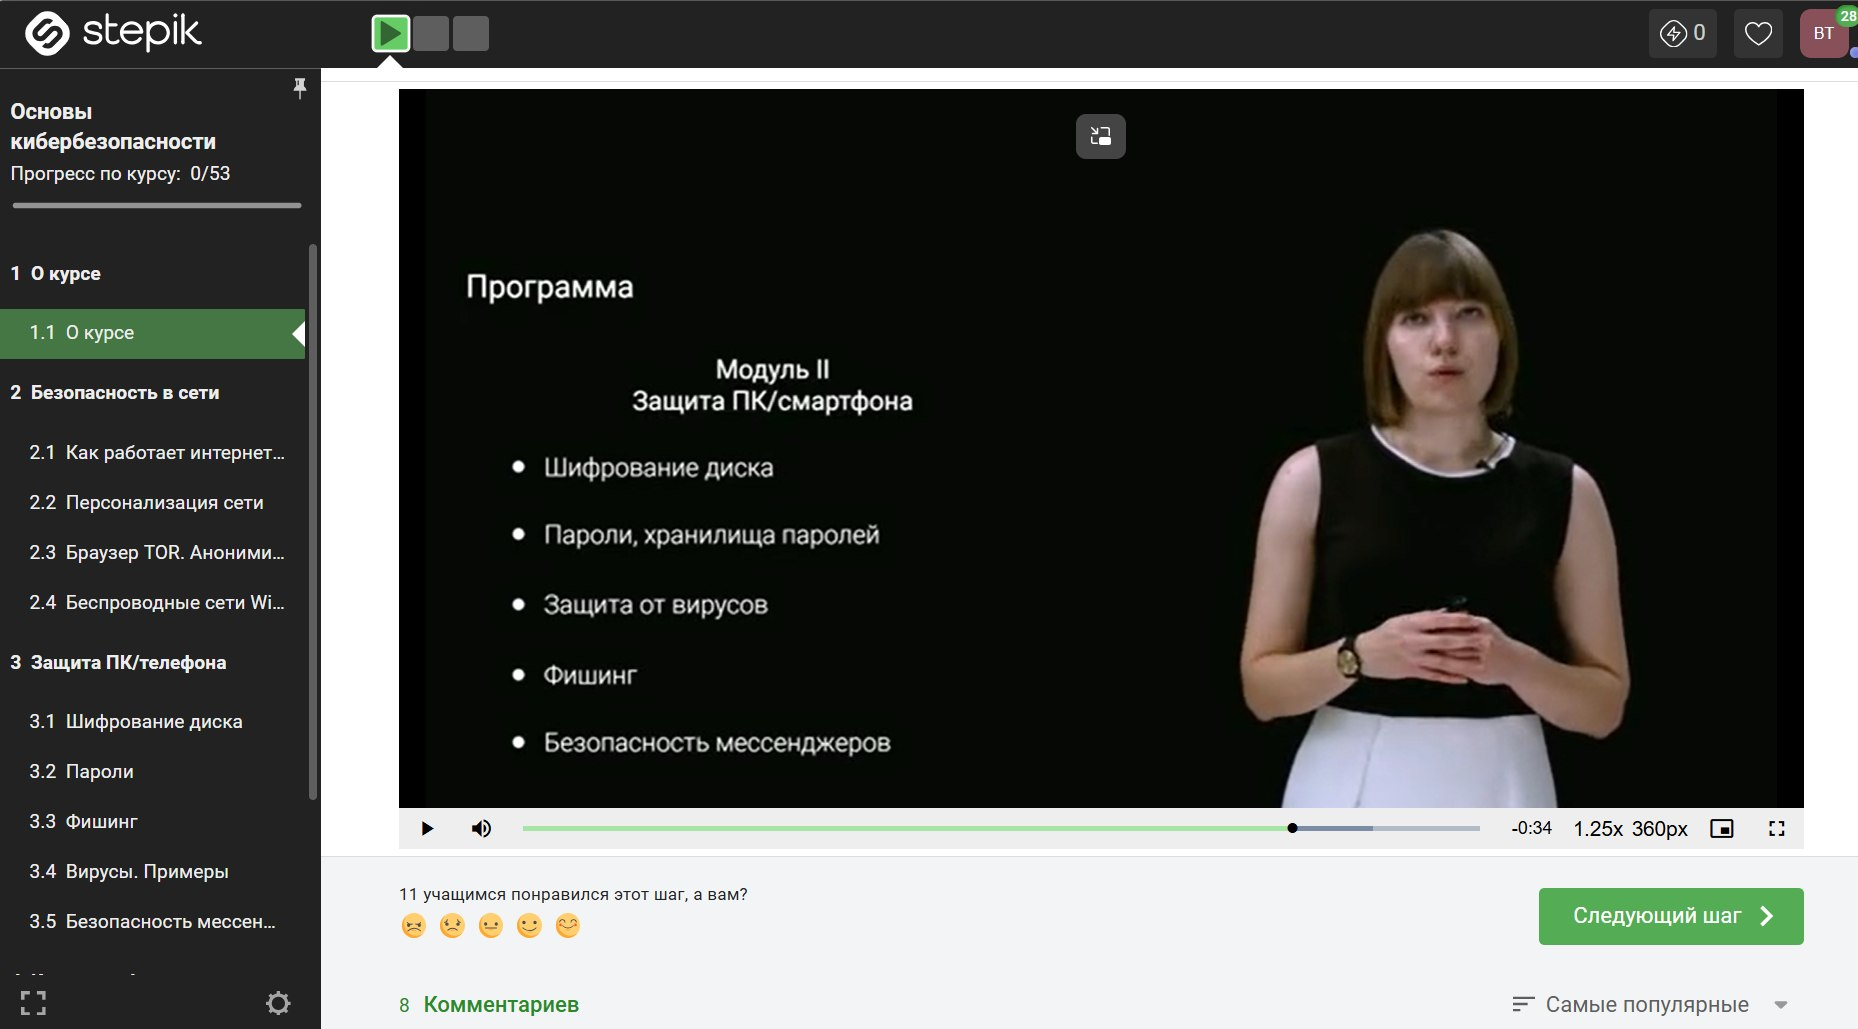
\includegraphics[width=0.7\textwidth,height=\textheight]{image/1.jpg}
\end{frame}

\begin{frame}{Безопасность в сети}
\phantomsection\label{ux431ux435ux437ux43eux43fux430ux441ux43dux43eux441ux442ux44c-ux432-ux441ux435ux442ux438}
Проходим первые задания на тему \enquote{Как работает интернет:базовые
протоколы}

(\textbf{?@fig-002}).
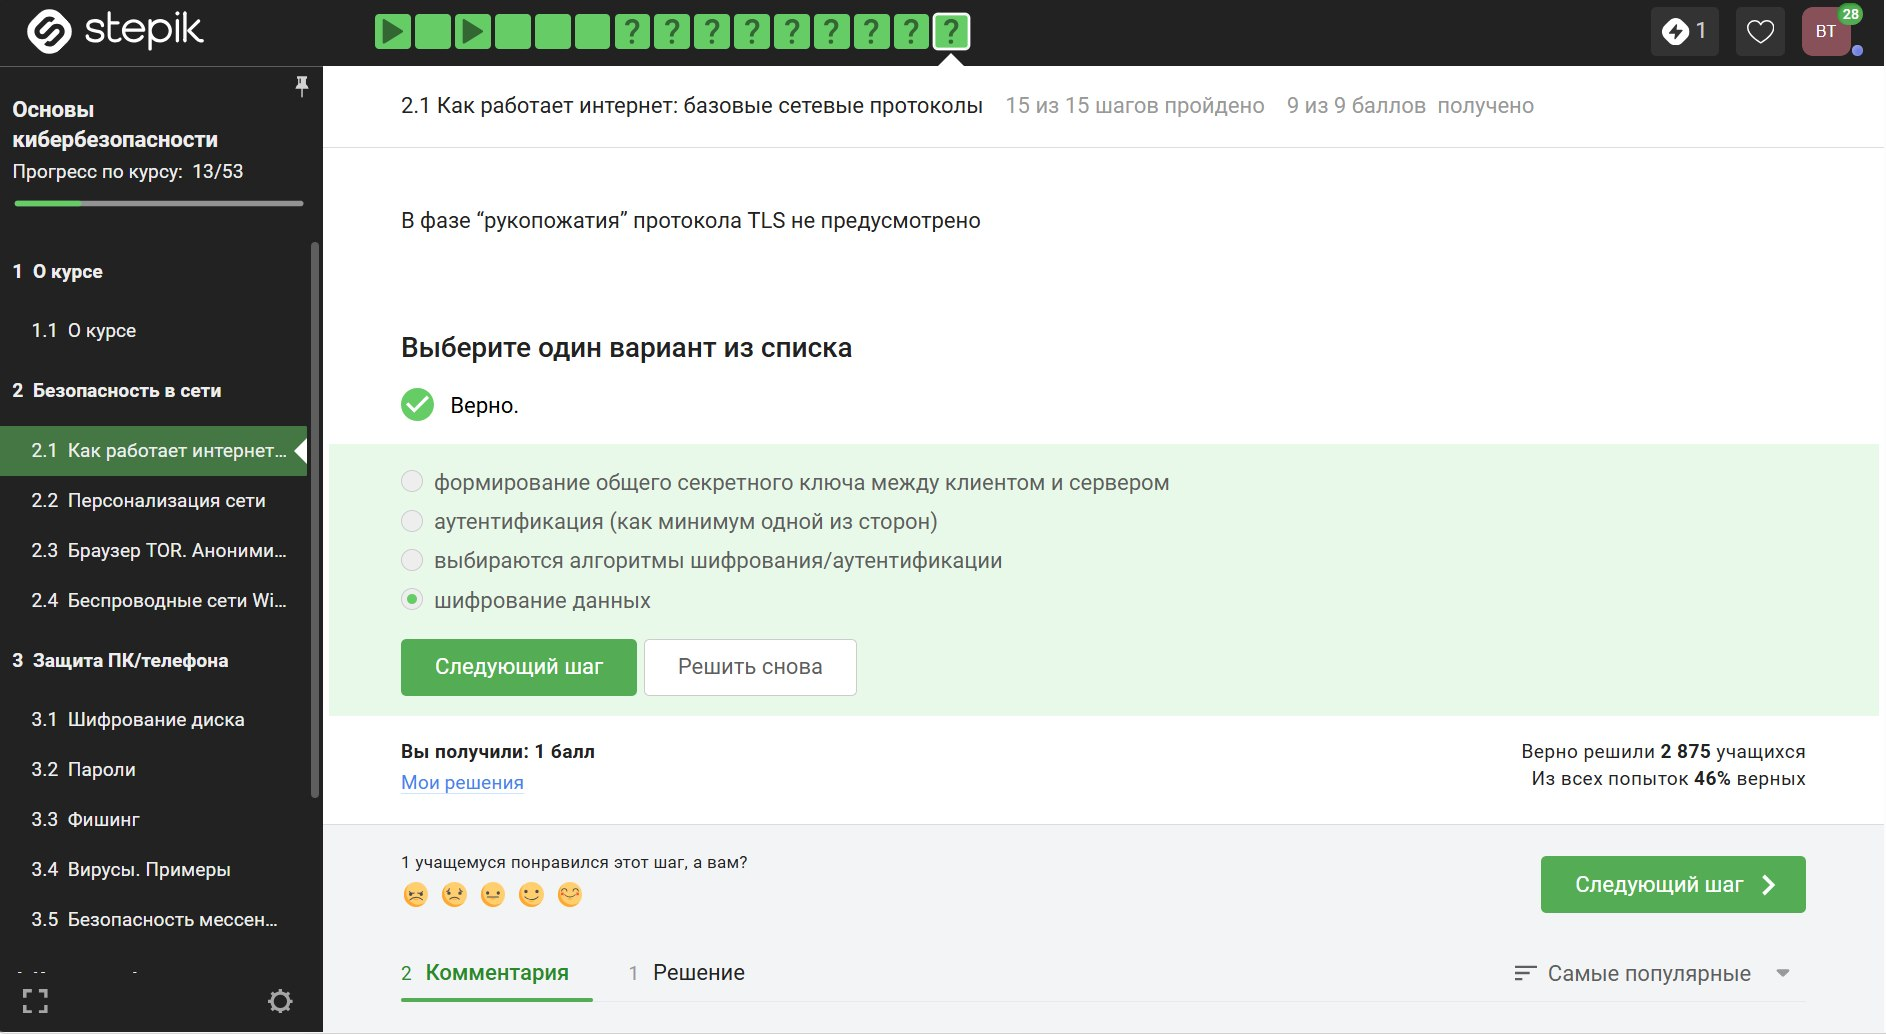
\includegraphics[width=0.7\textwidth,height=\textheight]{image/2.jpg}
\end{frame}

\begin{frame}{Персонализация в сеети}
\phantomsection\label{ux43fux435ux440ux441ux43eux43dux430ux43bux438ux437ux430ux446ux438ux44f-ux432-ux441ux435ux435ux442ux438}
Дплее выполняем задания связанные с персонализацией в сети

(\textbf{?@fig-003}).
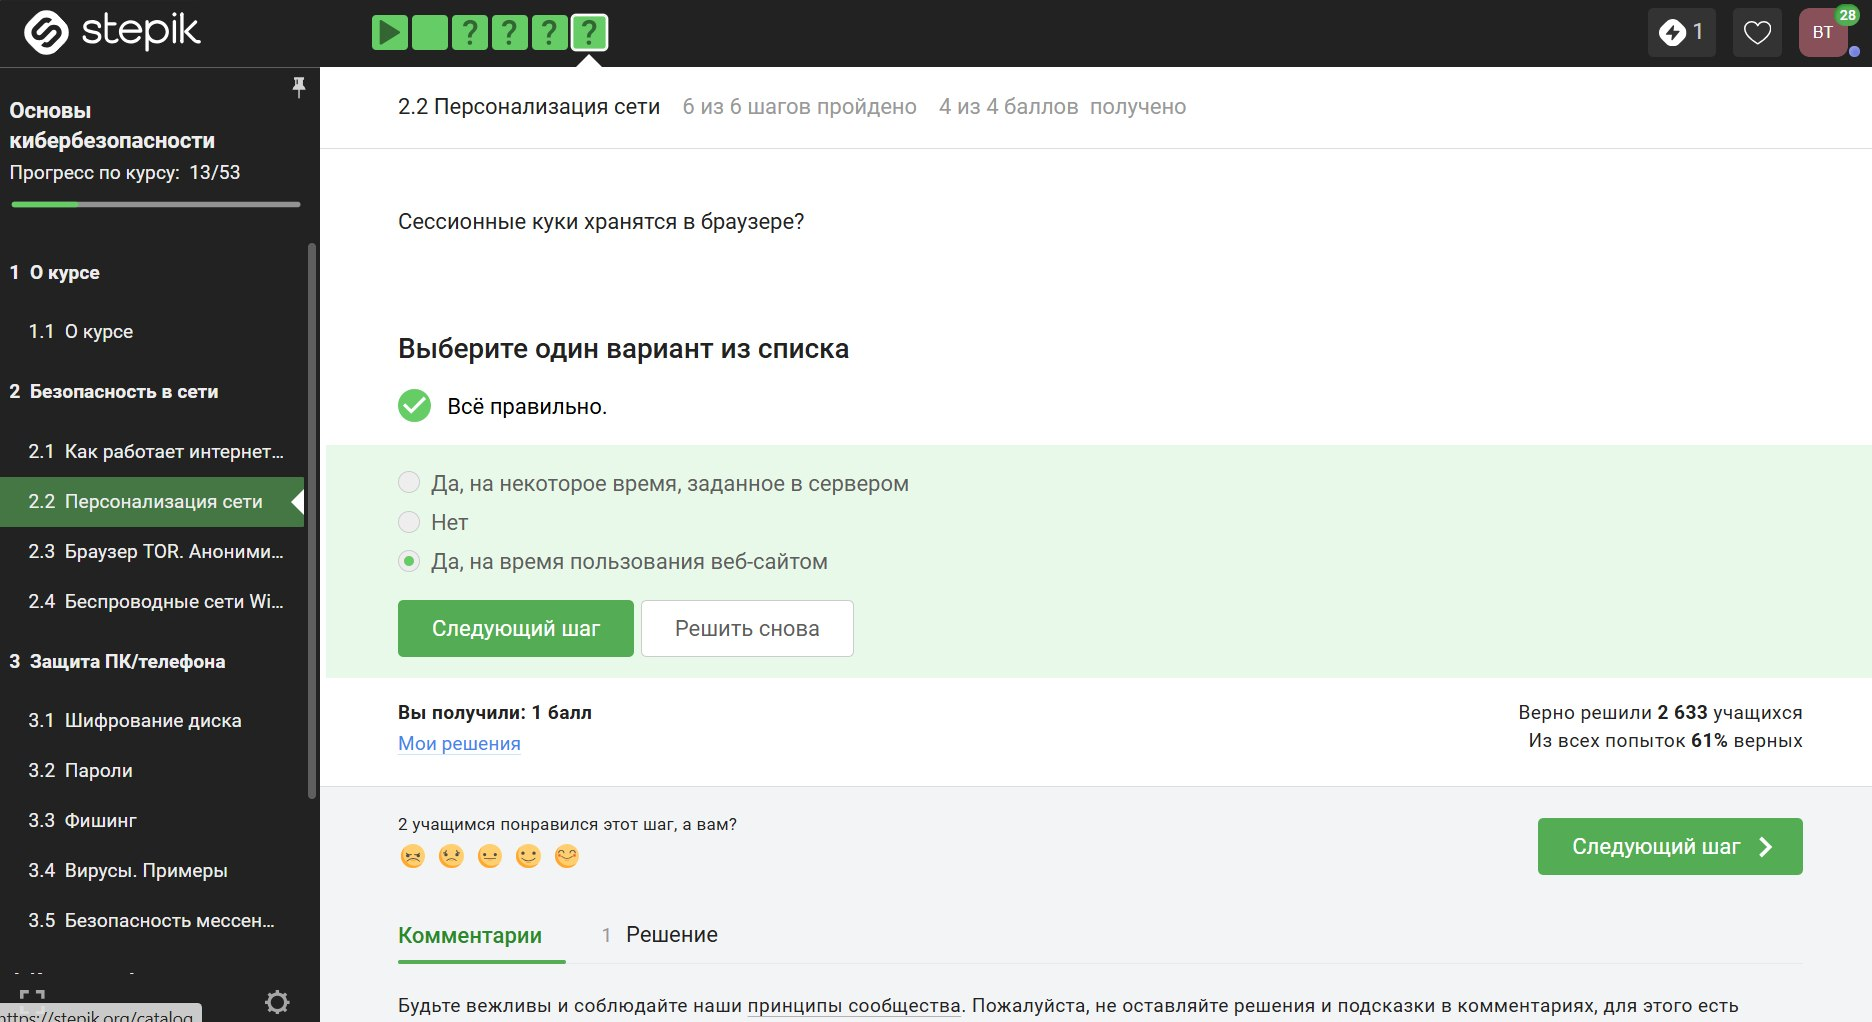
\includegraphics[width=0.7\textwidth,height=\textheight]{image/3.jpg}
\end{frame}

\begin{frame}{Браузер TOR и анонимицация}
\phantomsection\label{ux431ux440ux430ux443ux437ux435ux440-tor-ux438-ux430ux43dux43eux43dux438ux43cux438ux446ux430ux446ux438ux44f}
Знакомимся с браузером TOR и анонимицацией

(\textbf{?@fig-004}).
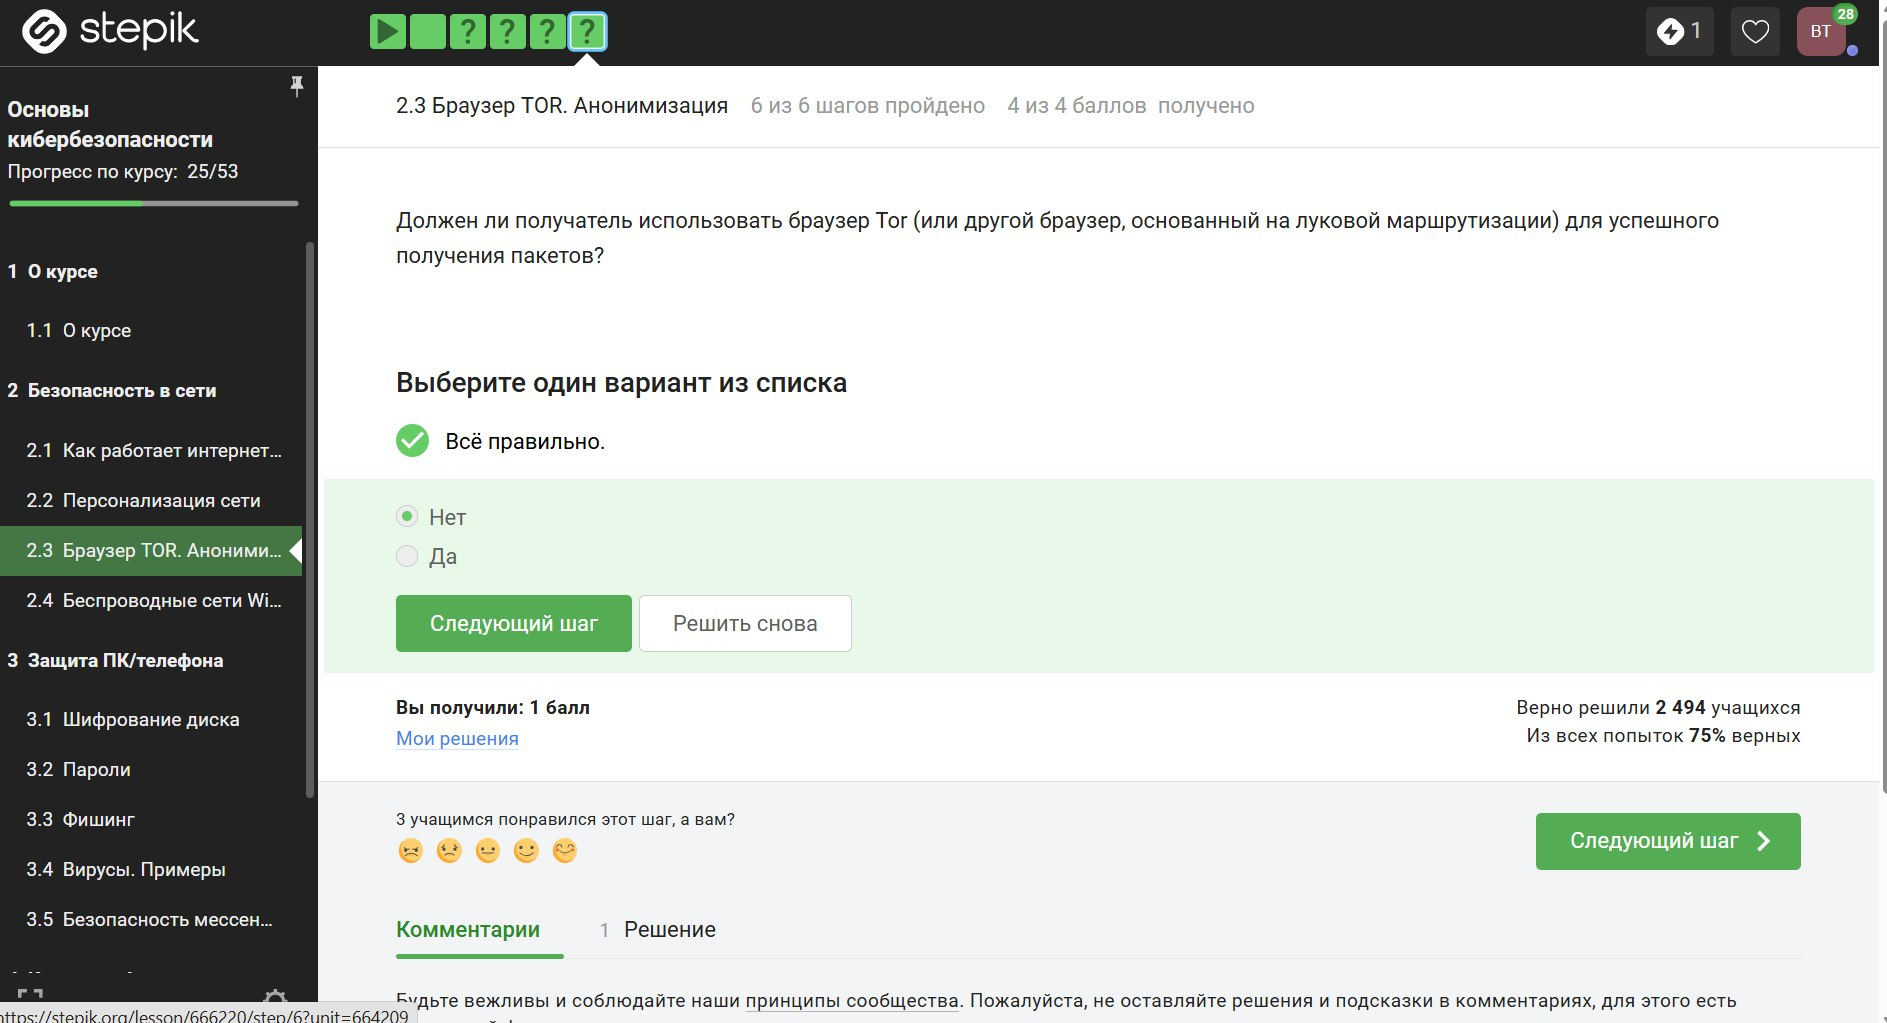
\includegraphics[width=0.7\textwidth,height=\textheight]{image/4.jpg}
\end{frame}

\begin{frame}{Беспроводные сети Wi-fi}
\phantomsection\label{ux431ux435ux441ux43fux440ux43eux432ux43eux434ux43dux44bux435-ux441ux435ux442ux438-wi-fi}
Затем переходим к беспроводным сетям Wi-fi

(\textbf{?@fig-005}).
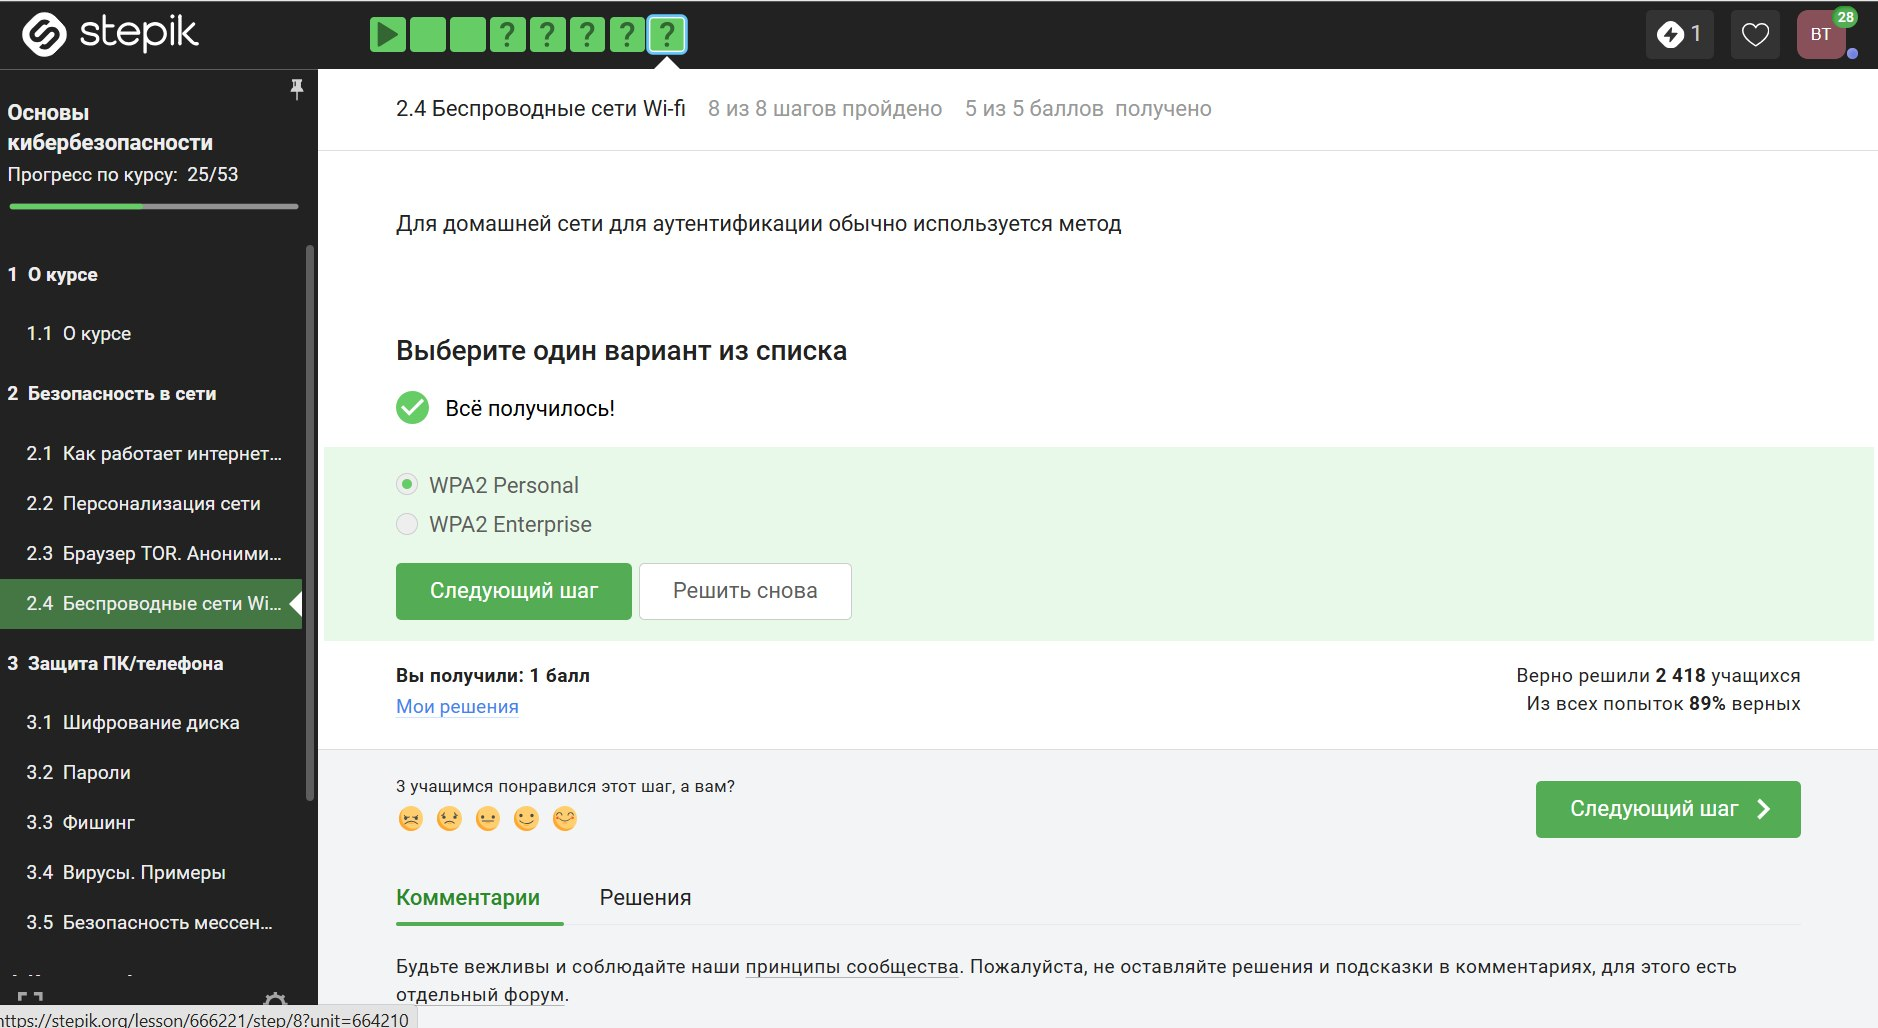
\includegraphics[width=0.7\textwidth,height=\textheight]{image/5.jpg}
\end{frame}

\begin{frame}{Защита ПК/телефона. Шифрование диска}
\phantomsection\label{ux437ux430ux449ux438ux442ux430-ux43fux43aux442ux435ux43bux435ux444ux43eux43dux430.-ux448ux438ux444ux440ux43eux432ux430ux43dux438ux435-ux434ux438ux441ux43aux430}
Выполняем задания на тему \enquote{Шифрование диска}. В этом пункте мы
узнаем как шифруются носители

(\textbf{?@fig-006}).
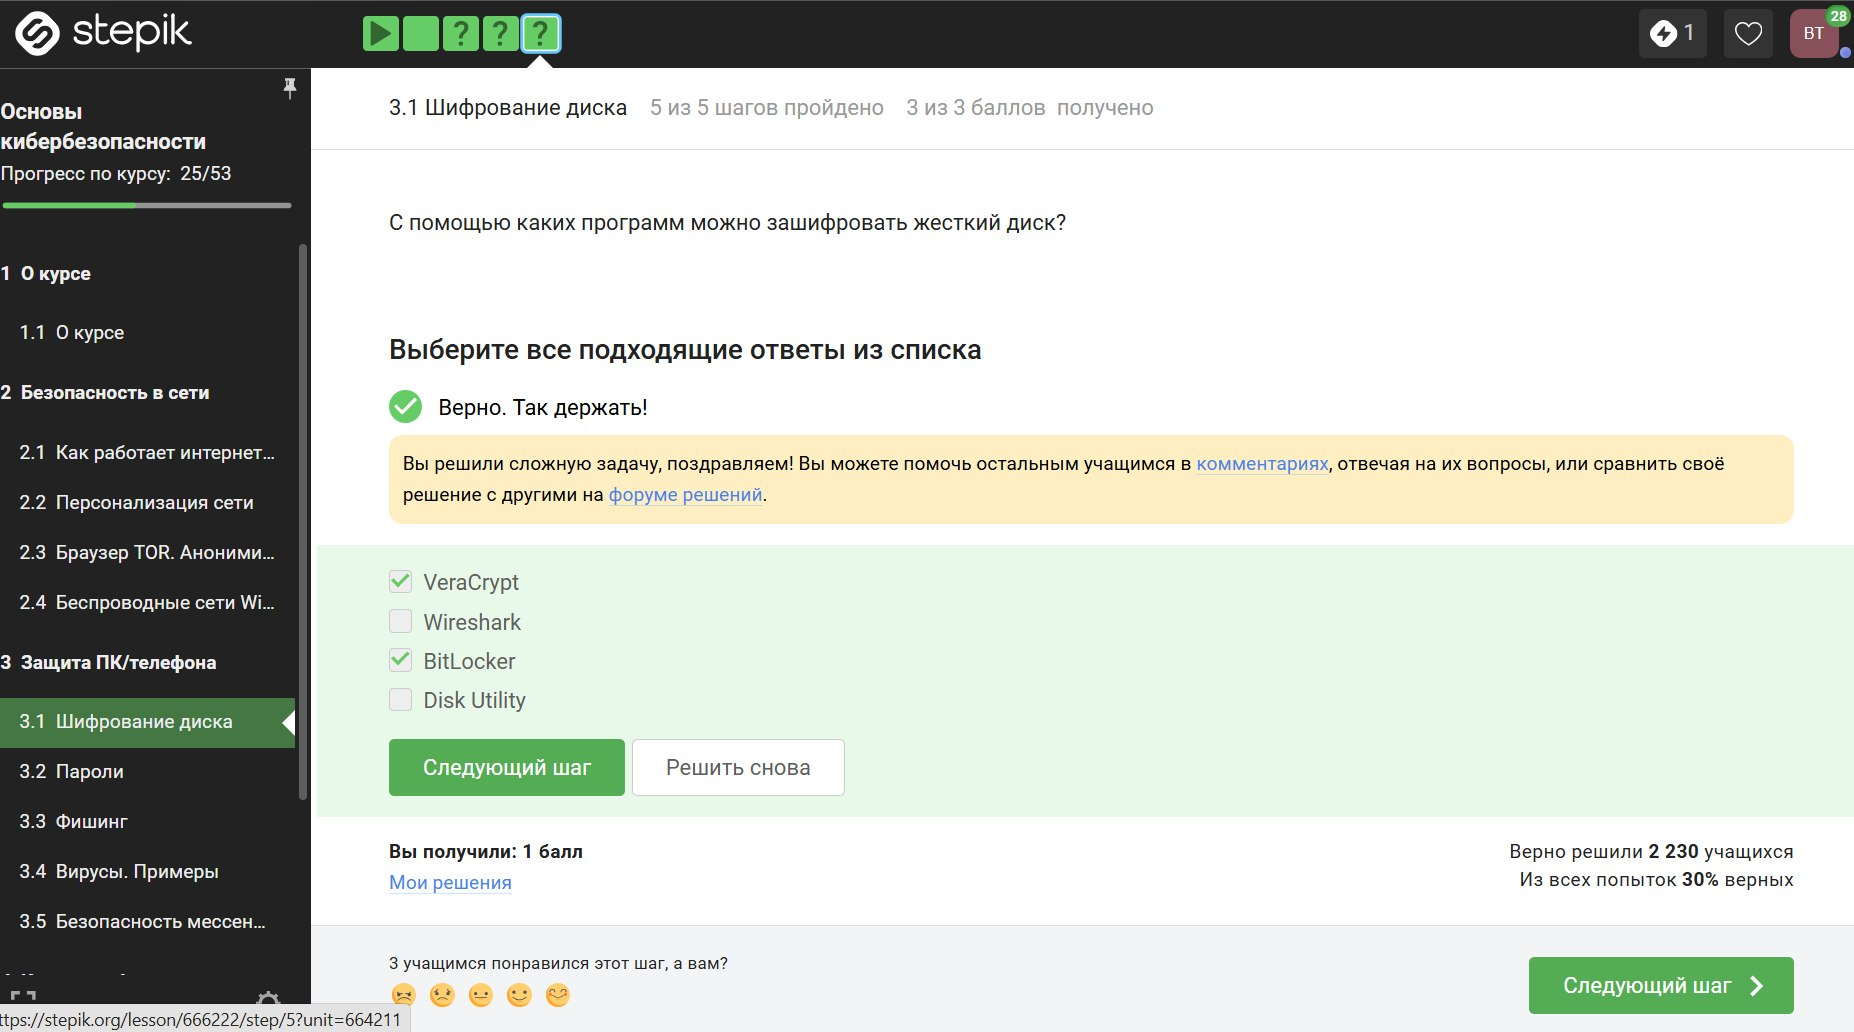
\includegraphics[width=0.7\textwidth,height=\textheight]{image/6.jpg}
\end{frame}

\begin{frame}{Пароли}
\phantomsection\label{ux43fux430ux440ux43eux43bux438}
Учимся обеспечивать наденость паролей и где их парвильно хранить

(\textbf{?@fig-007}).
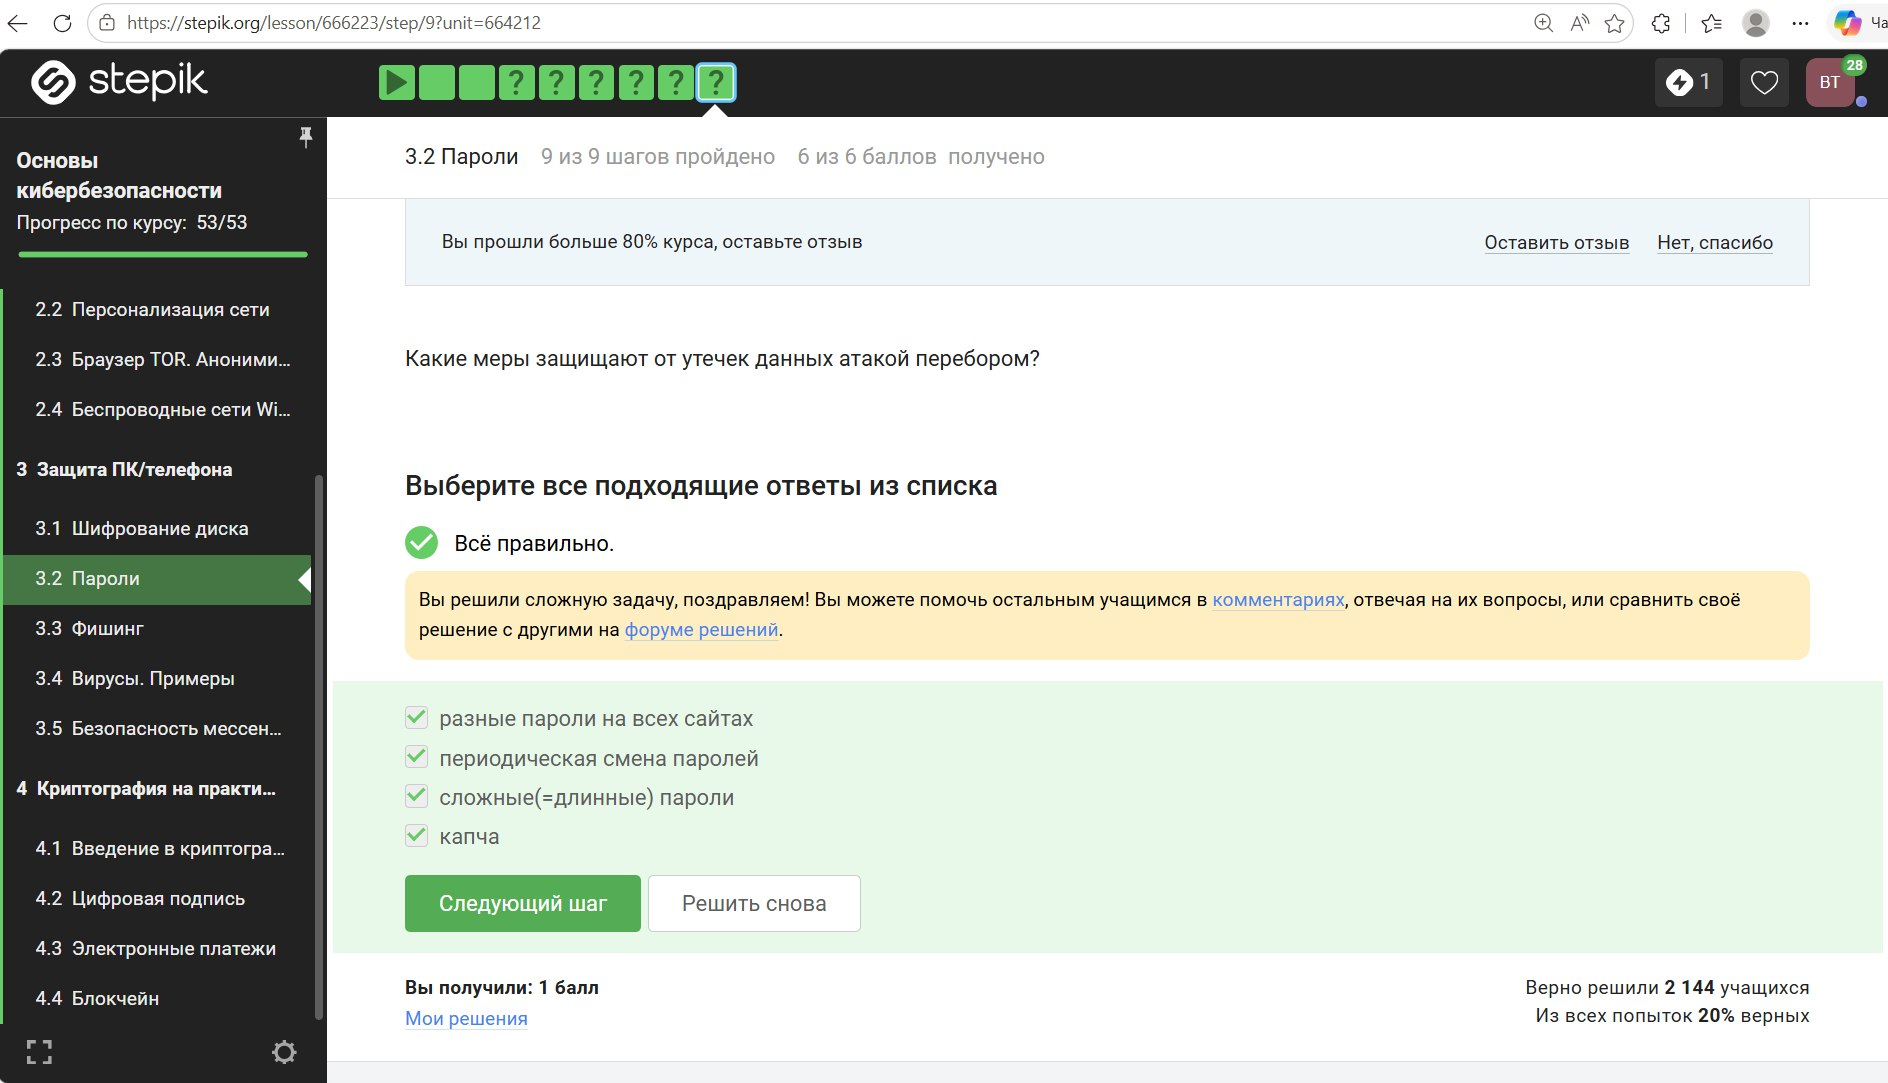
\includegraphics[width=0.7\textwidth,height=\textheight]{image/7.jpg}
\end{frame}

\begin{frame}{Фишинг}
\phantomsection\label{ux444ux438ux448ux438ux43dux433}
Рассматриваем, какие типы фишинговых рассылок бывают и как их можно
избежать.

(\textbf{?@fig-008}).
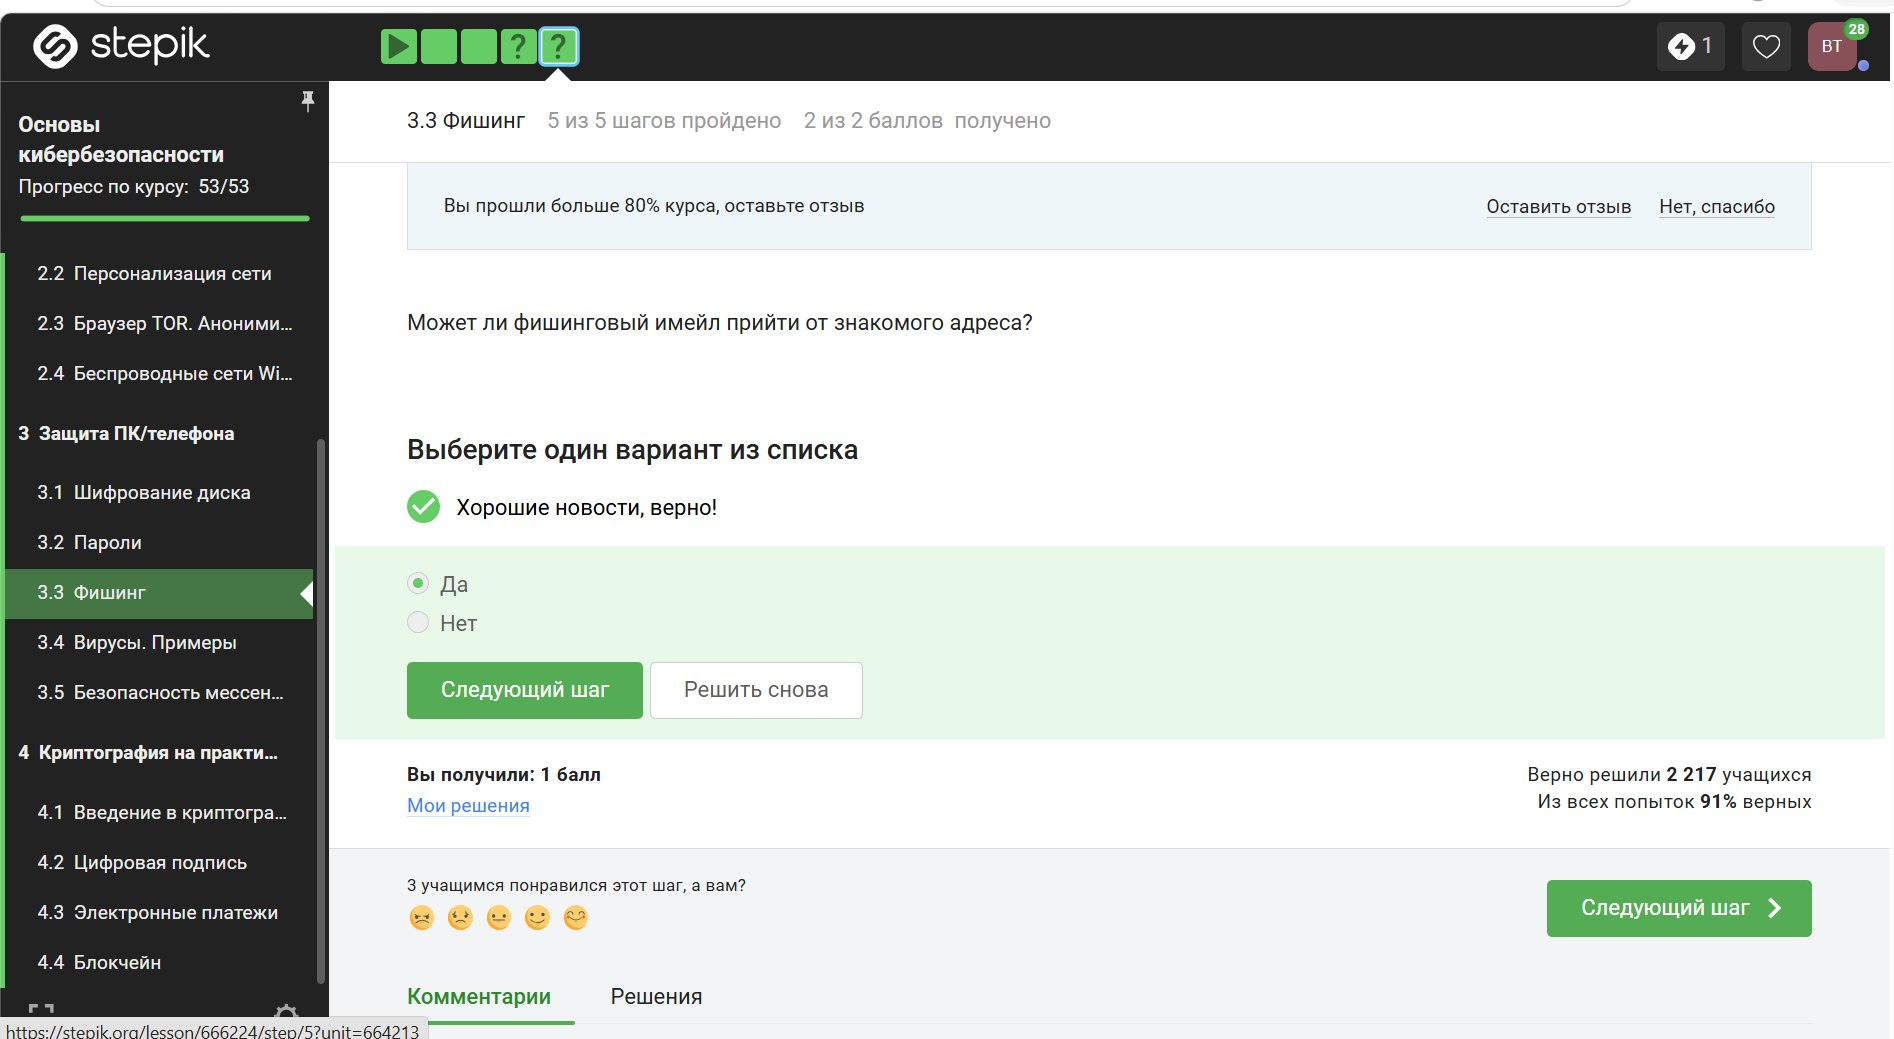
\includegraphics[width=0.7\textwidth,height=\textheight]{image/8.jpg}
\end{frame}

\begin{frame}{Вирусы}
\phantomsection\label{ux432ux438ux440ux443ux441ux44b}
Узнаем какие бывают вирусы и какой вред они могут наносить

(\textbf{?@fig-009}).
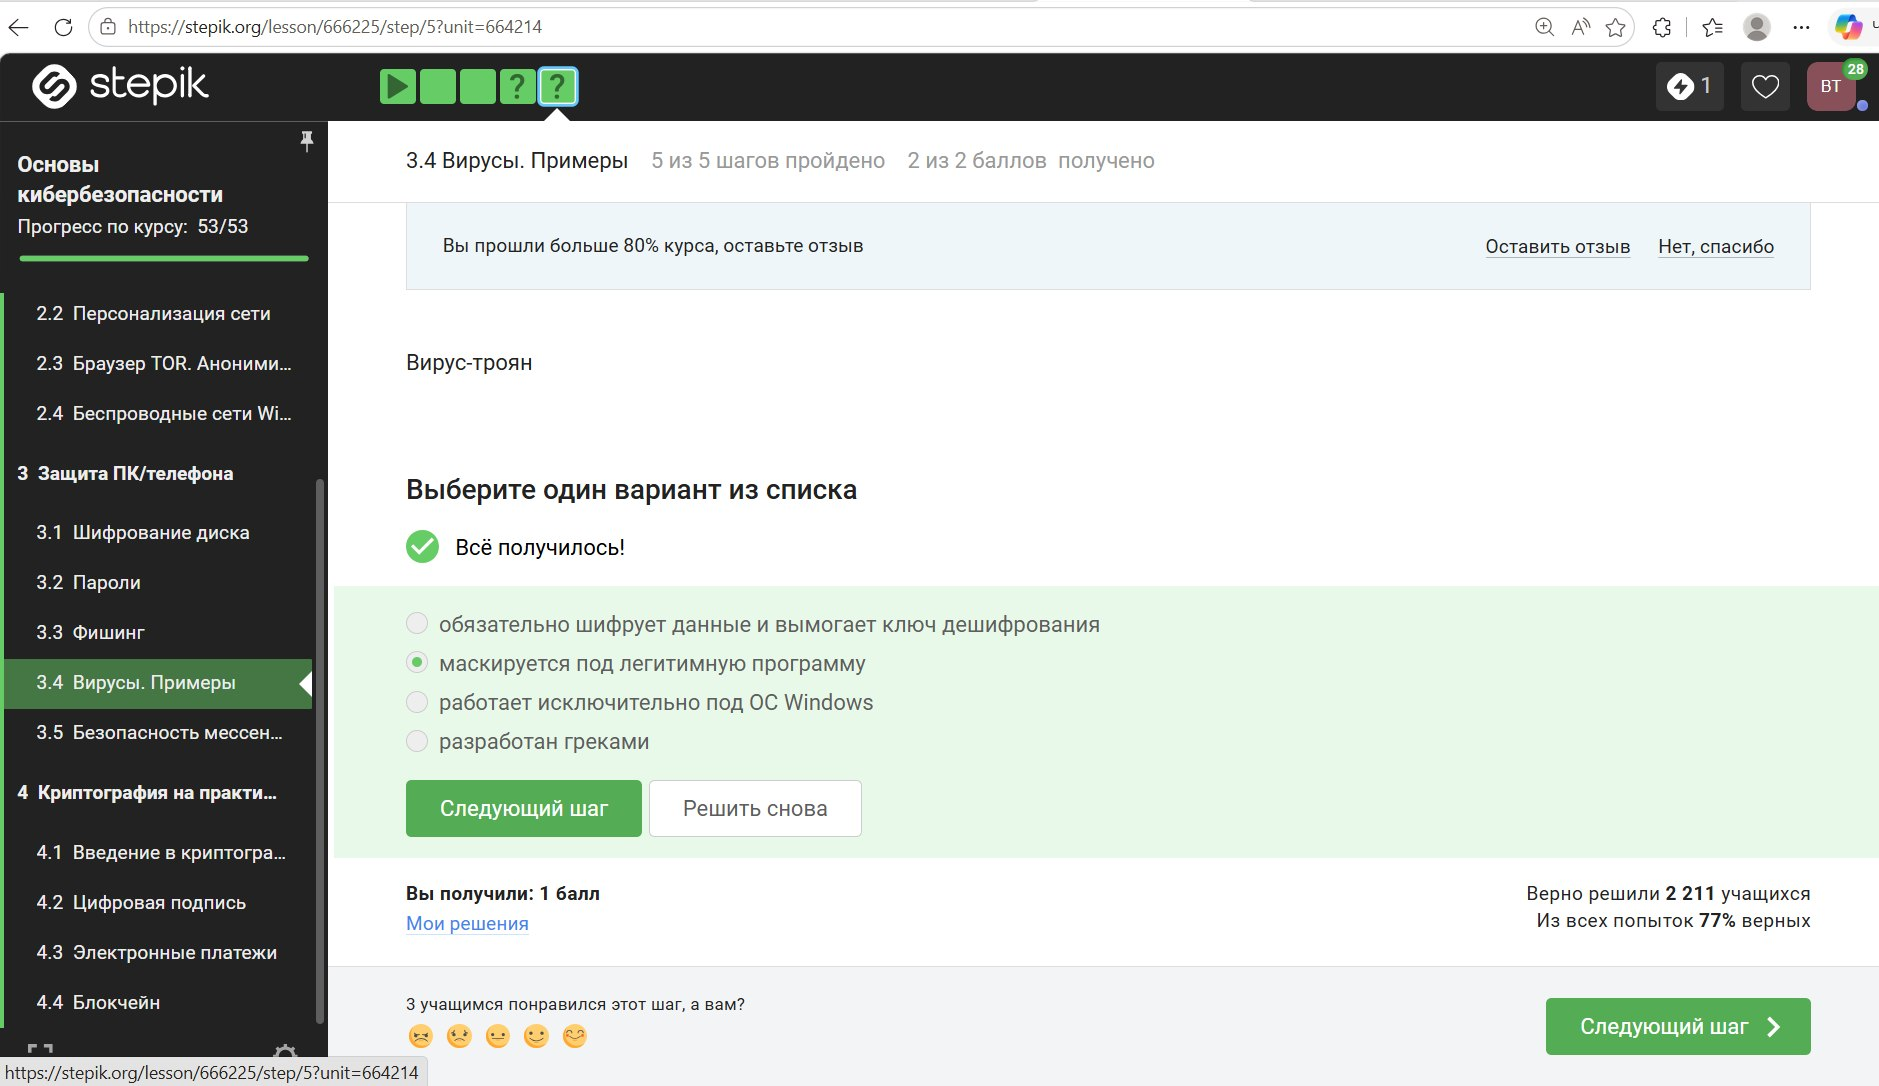
\includegraphics[width=0.7\textwidth,height=\textheight]{image/9.jpg}
\end{frame}

\begin{frame}{Безопасность мессенджеров}
\phantomsection\label{ux431ux435ux437ux43eux43fux430ux441ux43dux43eux441ux442ux44c-ux43cux435ux441ux441ux435ux43dux434ux436ux435ux440ux43eux432}
Узнаем как достигается безопасность сообщений в современных мессенджерах

(\textbf{?@fig-010}).
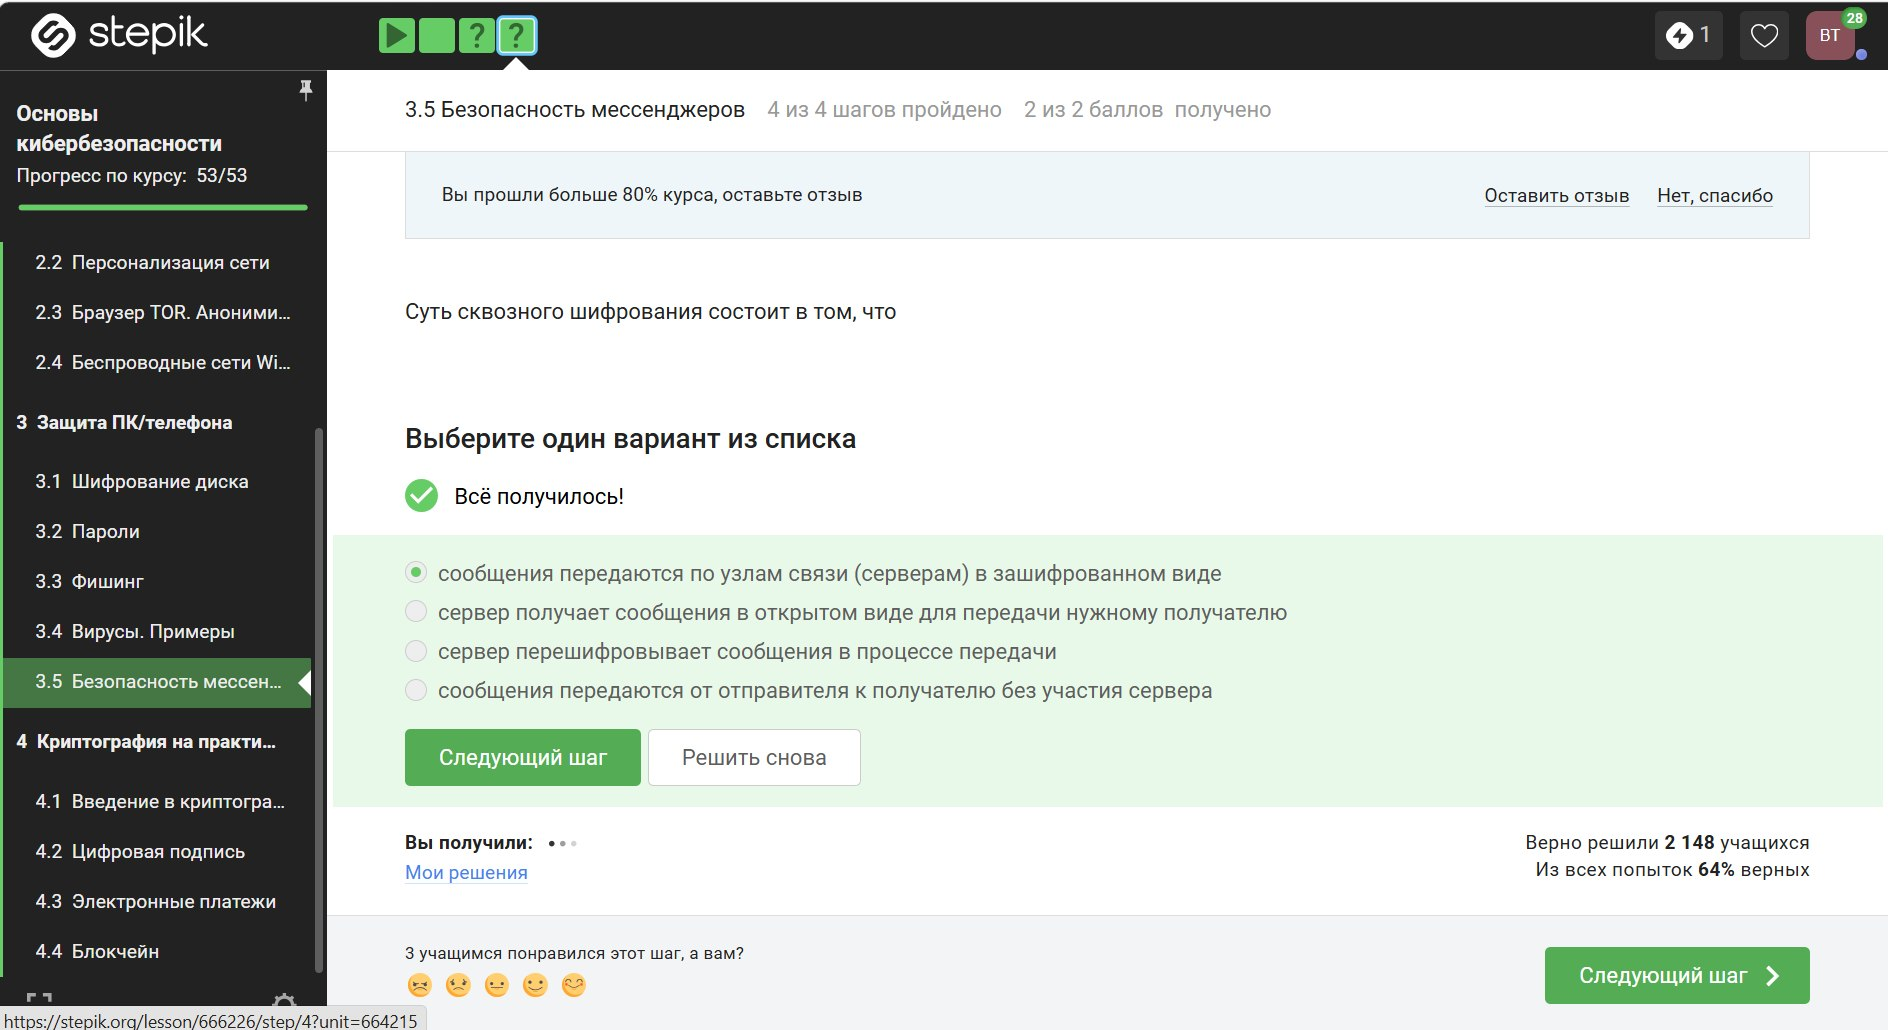
\includegraphics[width=0.7\textwidth,height=\textheight]{image/10.jpg}
\end{frame}

\begin{frame}{Криптография на практике. Введение в криптографию}
\phantomsection\label{ux43aux440ux438ux43fux442ux43eux433ux440ux430ux444ux438ux44f-ux43dux430-ux43fux440ux430ux43aux442ux438ux43aux435.-ux432ux432ux435ux434ux435ux43dux438ux435-ux432-ux43aux440ux438ux43fux442ux43eux433ux440ux430ux444ux438ux44e}
Узнаем какие бывают виды криптографии и как это применять
(\textbf{?@fig-011}).
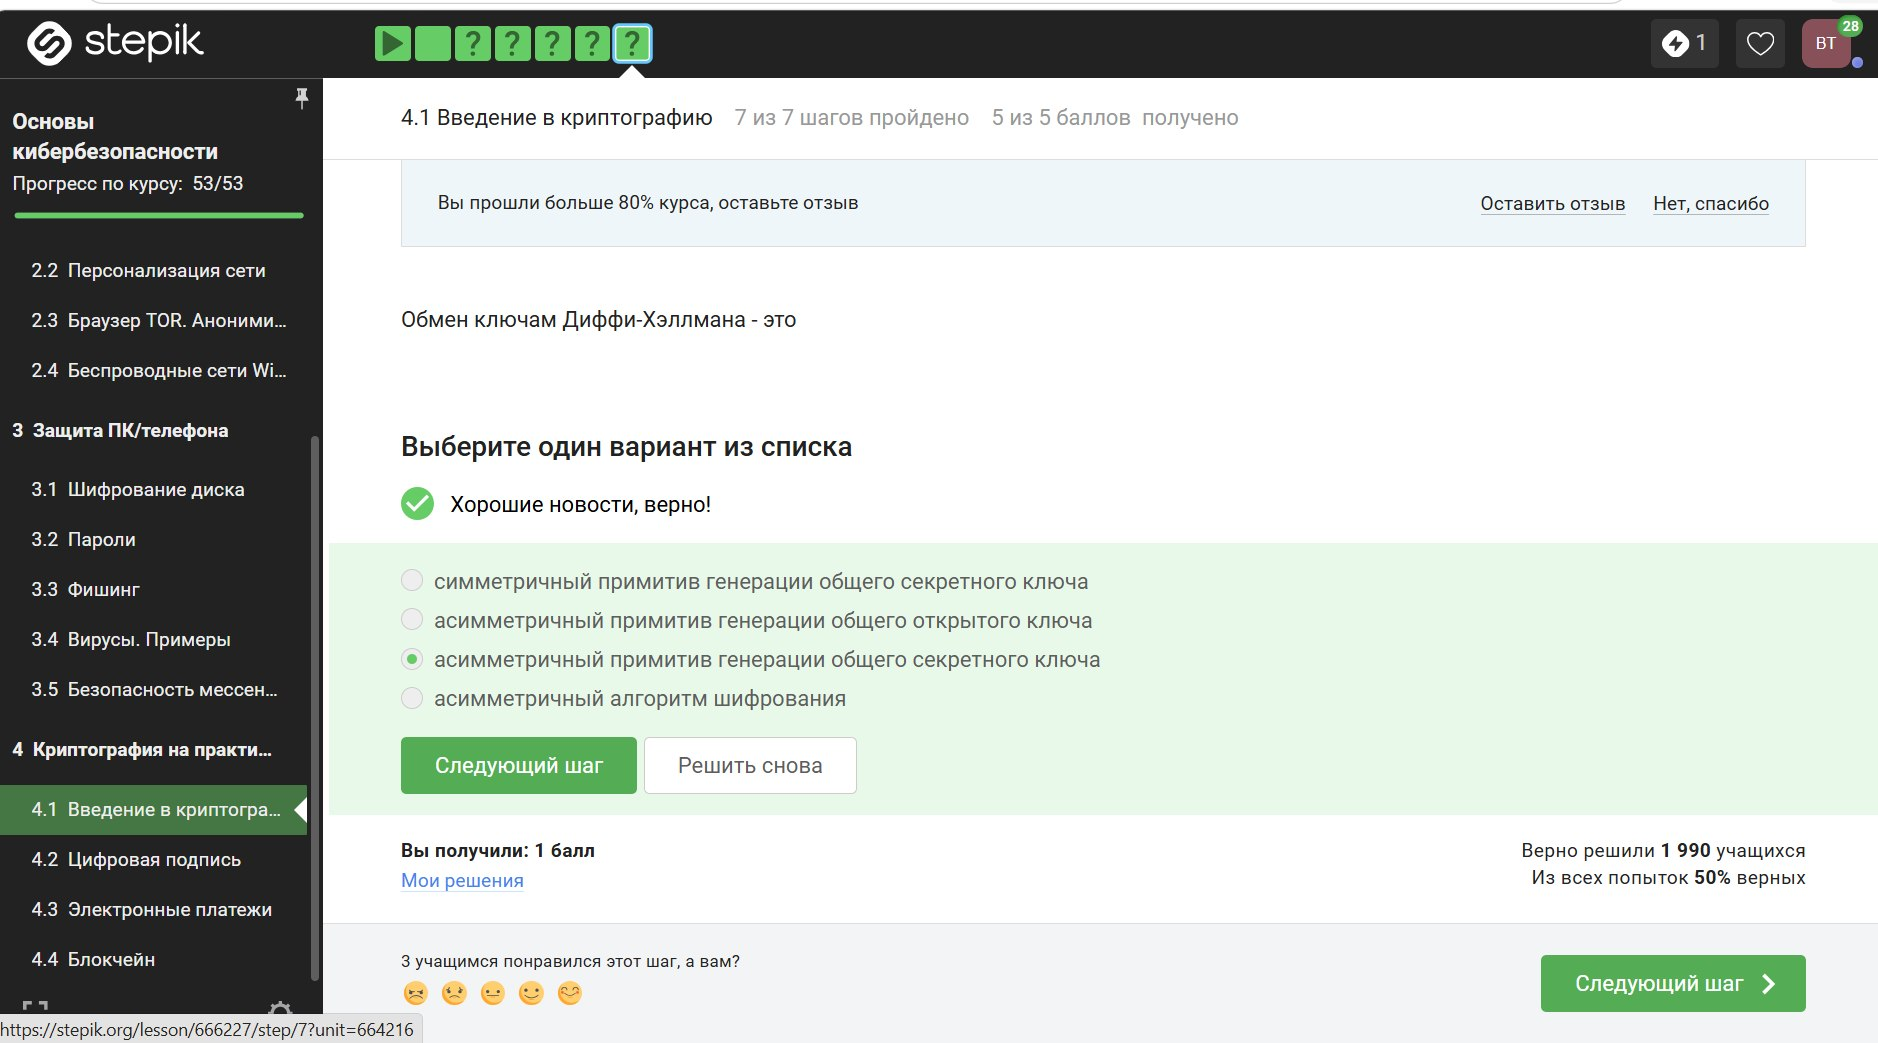
\includegraphics[width=0.7\textwidth,height=\textheight]{image/11.jpg}
\end{frame}

\begin{frame}{Цифровая подпись}
\phantomsection\label{ux446ux438ux444ux440ux43eux432ux430ux44f-ux43fux43eux434ux43fux438ux441ux44c}
Здесь мы знакомимся с применением электронно-цифровой подписи

(\textbf{?@fig-012}).
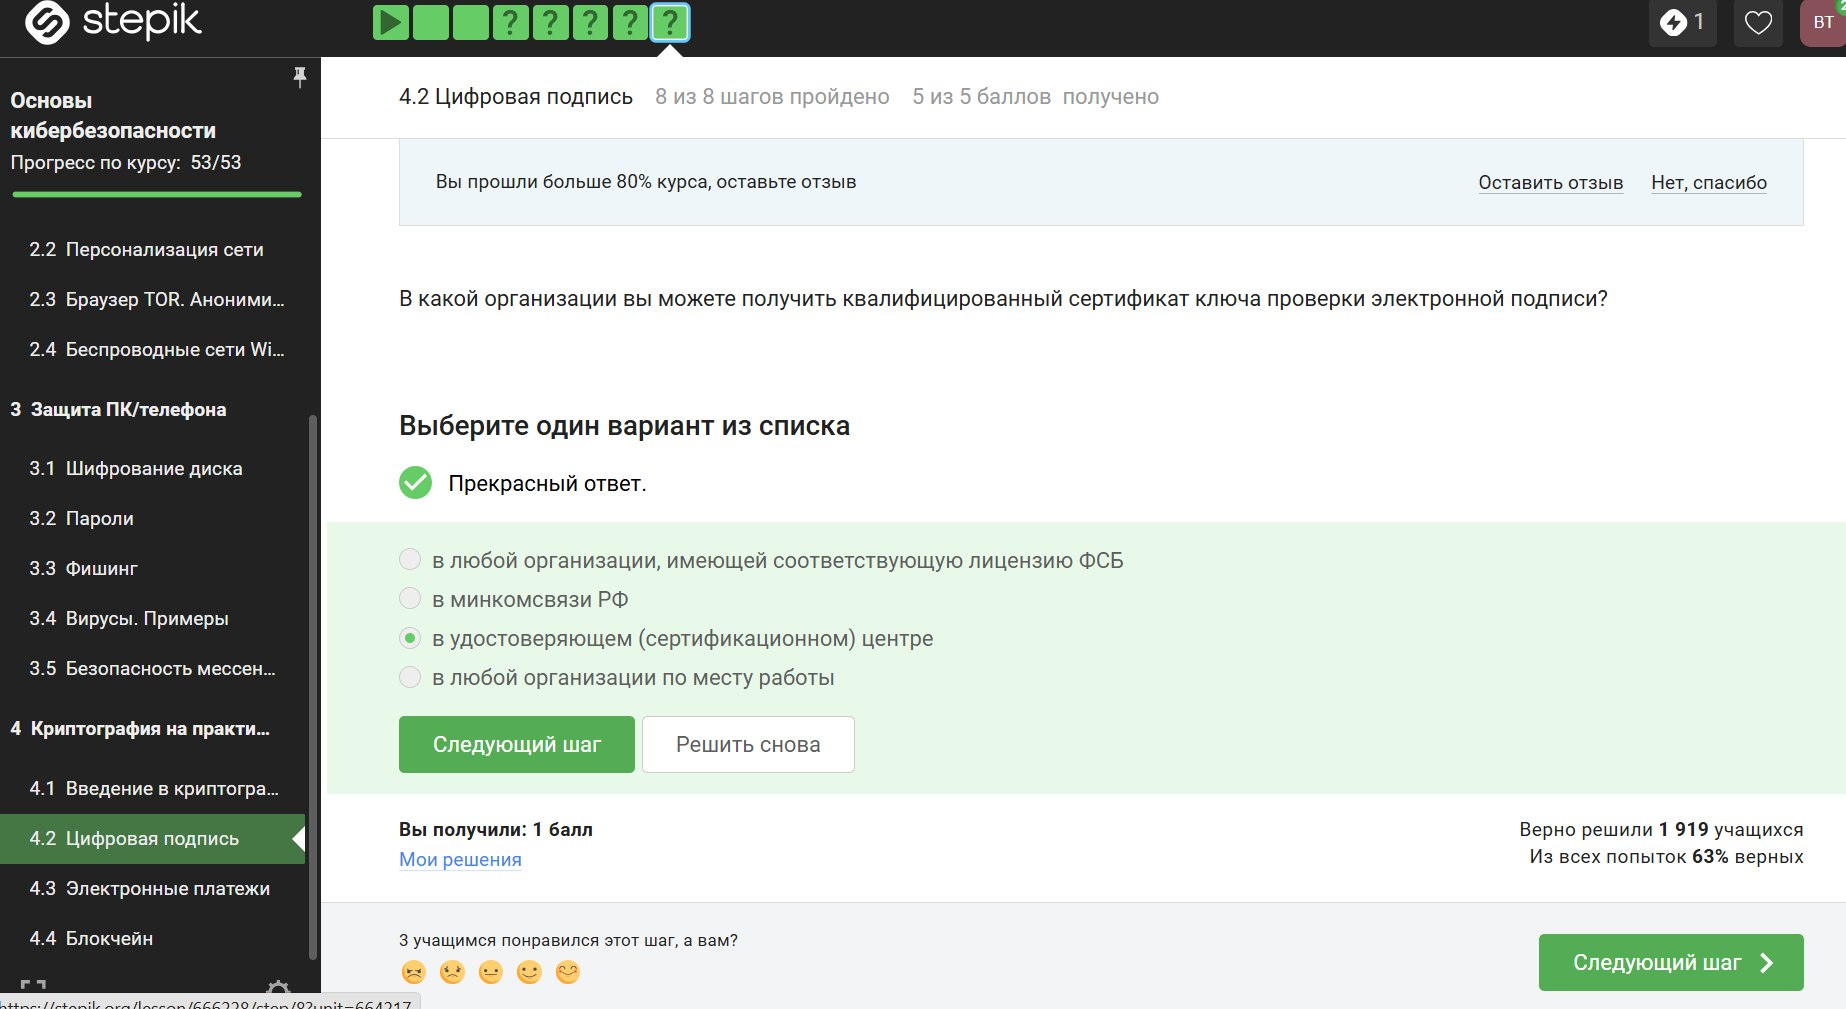
\includegraphics[width=0.7\textwidth,height=\textheight]{image/12.jpg}
\end{frame}

\begin{frame}{Электронные платежи}
\phantomsection\label{ux44dux43bux435ux43aux442ux440ux43eux43dux43dux44bux435-ux43fux43bux430ux442ux435ux436ux438}
Узнаем как работают электронные платежи

(\textbf{?@fig-013}).
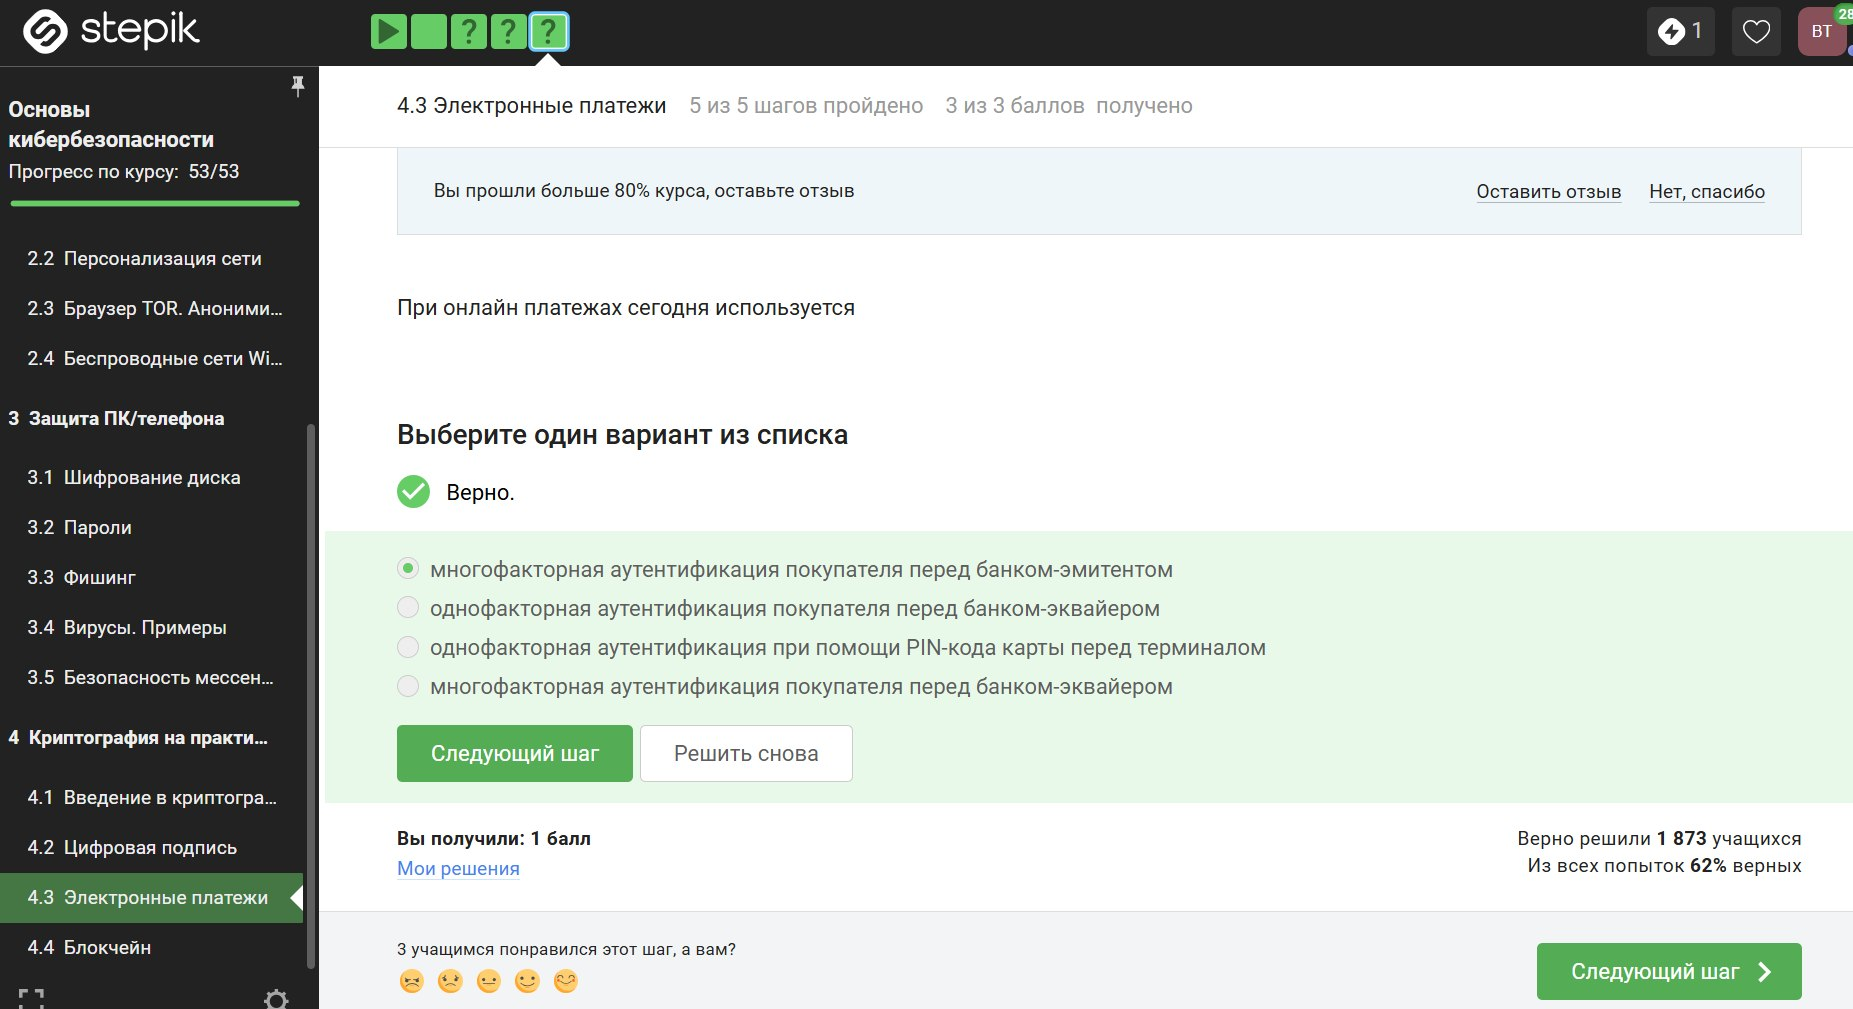
\includegraphics[width=0.7\textwidth,height=\textheight]{image/13.jpg}
\end{frame}

\begin{frame}{блкчейн}
\phantomsection\label{ux431ux43bux43aux447ux435ux439ux43d}
Разбираем систему блокчейн

(\textbf{?@fig-014}).
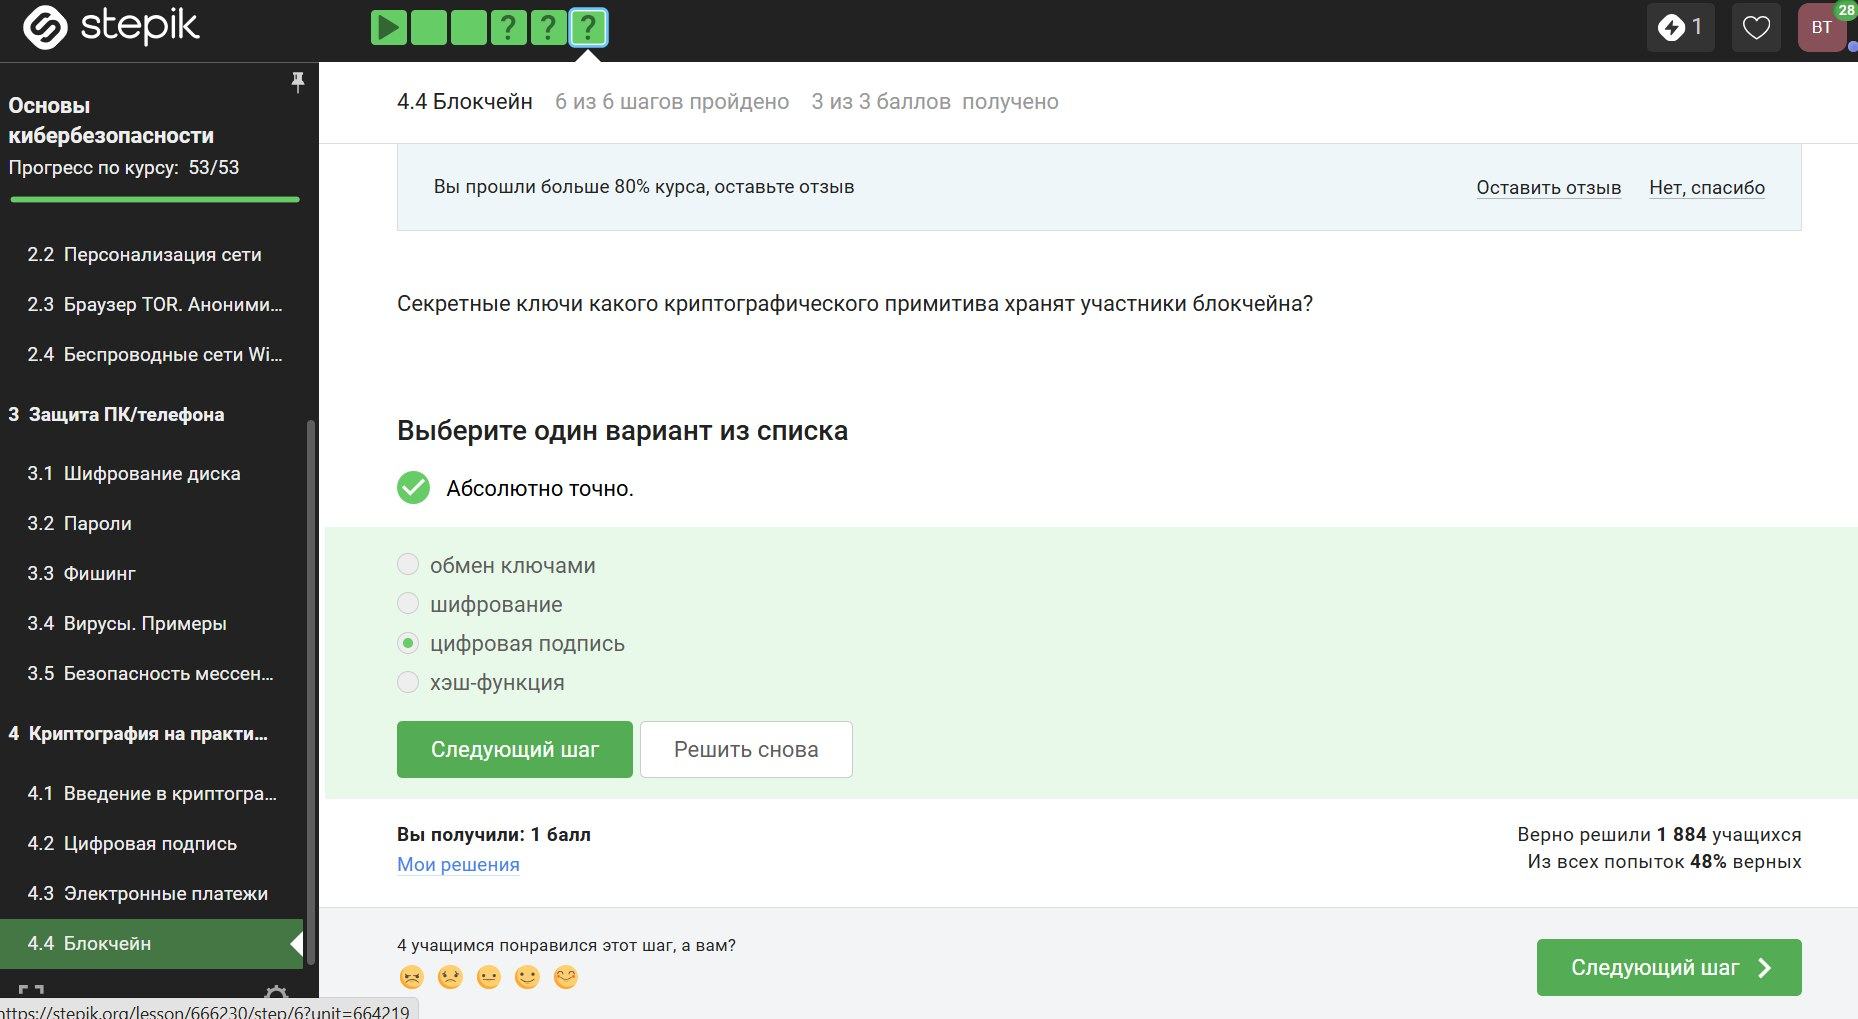
\includegraphics[width=0.7\textwidth,height=\textheight]{image/14.jpg}
\end{frame}

\begin{frame}{завершение курса}
\phantomsection\label{ux437ux430ux432ux435ux440ux448ux435ux43dux438ux435-ux43aux443ux440ux441ux430}
На этом завершаем прохождение курса

(\textbf{?@fig-015}).

\includegraphics[width=0.7\textwidth,height=\textheight]{image/15.jpg}
\end{frame}

\begin{frame}{Результаты}
\phantomsection\label{ux440ux435ux437ux443ux43bux44cux442ux430ux442ux44b}
Я прошла курс \enquote{Основы кибербезопасности}, во время прохождения
которого я получила навыки обеспечения безопасности в сети, узнала как
правильно защитить свои устройства и получила навыки криптографии
\end{frame}

\begin{frame}[fragile]{Код для формата \texttt{pdf}}
\phantomsection\label{ux43aux43eux434-ux434ux43bux44f-ux444ux43eux440ux43cux430ux442ux430-pdf}
\begin{Shaded}
\begin{Highlighting}[]
\FunctionTok{slide\_level}\KeywordTok{:}\AttributeTok{ }\DecValTok{2}
\FunctionTok{aspectratio}\KeywordTok{:}\AttributeTok{ }\DecValTok{169}
\FunctionTok{section{-}titles}\KeywordTok{:}\AttributeTok{ }\CharTok{true}
\FunctionTok{theme}\KeywordTok{:}\AttributeTok{ metropolis}
\end{Highlighting}
\end{Shaded}
\end{frame}

\begin{frame}[fragile]{Код для формата \texttt{html}}
\phantomsection\label{ux43aux43eux434-ux434ux43bux44f-ux444ux43eux440ux43cux430ux442ux430-html}
\begin{itemize}[<+->]
\tightlist
\item
  Тема задаётся в файле \texttt{Makefile}
\end{itemize}

\begin{Shaded}
\begin{Highlighting}[]
\NormalTok{REVEALJS\_THEME = beige}
\end{Highlighting}
\end{Shaded}
\end{frame}




\end{document}
